%\section*{Collaborators}
%List all your collaborators.

\documentclass[11pt]{article}

\usepackage[margin=1in]{geometry}
\usepackage{amsmath,amsthm,amssymb}
\usepackage{color}
\usepackage{lipsum} % for filler text
\usepackage{fancyhdr}
\pagestyle{fancy}
\usepackage{enumitem}
\usepackage{graphicx}

\newenvironment{problem}[2][Problem]{\begin{trivlist}
\item[\hskip \labelsep {\bfseries #1}\hskip \labelsep {\bfseries #2.}]}{\end{trivlist}}

\fancyhead{} % clear all header fields
\renewcommand{\headrulewidth}{0pt} % no line in header area
\fancyfoot{} % clear all footer fields
\newcommand\tab[1][1cm]{\hspace*{#1}}
\fancyfoot[LE,RO]{\thepage}           % page number in "outer" position of footer line
\fancyfoot[RE,LO]{Aashish Dhakal} %your name in footer line

\begin{document}
%\lipsum[1-20]
\title{CS 572(Assignment 5)} %replace X with the appropriate number
\author{Aashish Dhakal\\ %replace with your name
aashish@iastate.edu\\%replace with username
 }      %if necessary, replace with your course title
\date{}


\maketitle
\section*{}

\textbf{Problem 7.2}
\begin{enumerate}[label=(\alph*)]
  \item We are going to use the following syntax and semantics as our knowledge base:\\
  $K_1$ = the unicorn is mythical \\
  $K_2$ = the unicorn is mortal \\
  $K_3$ = the unicorn is mammal \\
  $K_4$ = the unicorn has horn \\
  $K_5$ = the unicorn is magical \\ \\
  NOTE: $\daleth$ symbol means "NOT" \\
  Now we can represent all the conditions as follows:
    \begin{enumerate}
      \item $P_1: K_1 \Rightarrow \daleth K_2$
      \item $P_2: \daleth K_1 \Rightarrow (K_2 \wedge K_3$)
      \item $P_3: (\daleth K_2 \vee K_3) \Rightarrow K_4$
      \item $P_4: K_4 \Rightarrow K_5$
    \end{enumerate}
  Mythical:\\
  Assume that the Unicorn is Mythical is $True$ i.e. $K_1$ is true.\\
  Now we can easily say that: \\
  $K_2$ is $True$,
  $K_3$ is $True$,
  $K_4$ is $True$,
  $K_5$ is $True$\\
  Thus, The Knowledge base is satisfied.\\ \\
  Assume that the Unicorn is Mythical is $False$ i.e. $K_1$ is False.\\
  Now we can easily say that: \\
  $K_2$ is $False$,
  $K_3$ is $True$,
  $K_4$ is $True$,
  $K_5$ is $True$ \\
  Thus, The Knowledge base is satisfied.\\
  As the knowledge base is satisfied for both the statemets i.e. Unicorn being mythical and not mythical,
  we cannot infer anything. Hence, Proved!\\ \\
  Magical:\\
  Transforming the Knowledge Base into $CNF$\\
  $P_1: \daleth K_1 \vee  K_2 \\
  P_2: (K_1 \vee \daleth K_2) \wedge (K_1 \vee K_3) \\
  P_3: (\daleth K_2 \vee  K_4) \wedge (\daleth K_3 \vee  K_4) \\
  P_4: \daleth K_4 \vee  K_5$ \\ \\
  Now, lets separate the conjuct:\\
  $C_1: \daleth K_1 \vee  K_2 \\
  C_2: K_1 \vee \daleth K_2\\
  C_3: K_1 \vee K_3 \\
  C_4: \daleth K_2 \vee  K_4 \\
  C_5: \daleth K_3 \vee  K_4 \\
  C_6: \daleth K_4 \vee  K_5$ \\ \\

  Now let's add $\daleth P_5$, in order to prove or disprove that the Unicorn is Magical.\\
  $C_7: \daleth P_5$ \\ \\
  Using one $CNF$ rule on other we solve:\\
  $C_8: K_2 \vee  K_3$ ------ from $C_1$ and $C_3$ \\
  $C_9: K_3 \vee  K_4$ ------ from $C_8$ and $C_4$ \\
  $C_{10}: K_4$ ------ from $C_9$ and $C_5$ \\
  $C_{11}: K_5$ ------ from $C_{10}$ and $C_6$ \\
  $C_{12}: \{ \}$ ------ from $C_{11}$ and $C_7$ \\ \\
  So, by Proof of contradiction, we can say that Unicorn is Magical.\\ \\
  Again let's use the same $CNF$
  $C_1: \daleth K_1 \vee  K_2 \\
  C_2: K_1 \vee \daleth K_2\\
  C_3: K_1 \vee K_3 \\
  C_4: \daleth K_2 \vee  K_4 \\
  C_5: \daleth K_3 \vee  K_4 \\
  C_6: \daleth K_4 \vee  K_5$ \\ \\
  Now let's add $\daleth P_4$, in order to prove that the Unicorn is horned.\\
  $C_7: \daleth P_4$ \\ \\
  Using one $CNF$ rule on other we solve:\\
  $C_8: K_2 \vee  K_3$ ------ from $C_1$ and $C_3$ \\
  $C_9: K_3 \vee  K_4$ ------ from $C_8$ and $C_4$ \\
  $C_{10}: K_4$ ------ from $C_9$ and $C_5$ \\
  $C_{11}: \{ \}$ ------ from $C_{10}$ and $C_7$ \\ \\
  So, by Proof of contradiction, we can say that Unicorn is Horned.\\ \\ \\ \\ \\
\end{enumerate}
\textbf{Problem 7.18} \\
Given:
$[(Food \Rightarrow Party) \vee (Drinks \Rightarrow Party)] \Rightarrow [(Food \wedge Drinks) \Rightarrow Party]$ \\ \\
\textbf{a.} Lets use a Truth Table, with the notations as: \\
$[(F \Rightarrow P) \vee (D \Rightarrow P)] \Rightarrow [(F \wedge D) \Rightarrow P]$
\begin{figure}
  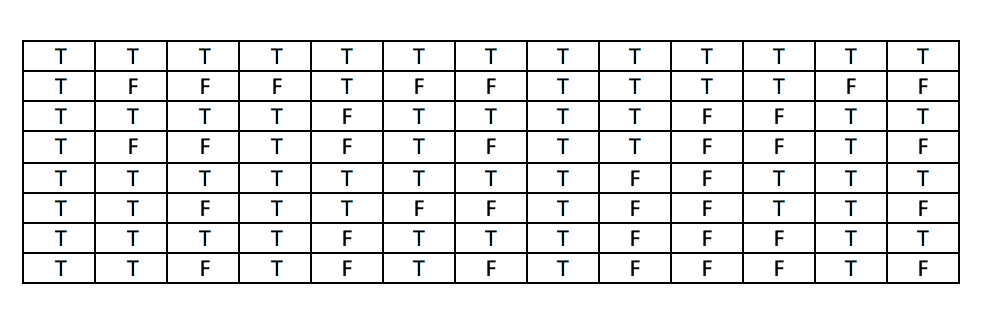
\includegraphics[width=\linewidth]{table.png}
  \caption{Truth Table}
\end{figure}
\\ So, the above truth table shows that the sentence is true, hence Valid. \\ \\
\textbf{b.} \\
Converting the LHS of main implication to $CNF$:\\
- $(Food \Rightarrow Party) \vee (Drinks \Rightarrow Party)$\\
- $(\daleth Food \vee Party) \vee (\daleth Drinks \vee Party)$ \\
- $(\daleth Food \vee Party \vee \daleth Drinks \vee Party)$ \\
- $(\daleth Food \vee \daleth Drinks \vee Party)$ \\ \\
Converting the RHS of main implication to $CNF$:\\
- $(Food \wedge Drinks) \Rightarrow Party$\\
- $\daleth (Food \wedge Drinks) \vee Party$\\
- $(\daleth Food \vee \daleth Drinks) \vee Party$ \\
- $\daleth Food \vee \daleth Drinks \vee Party$ \\ \\
Since we have $LHS = RHS$, we know that it is a valid statement and thus confirms to answer in Part a. \\ \\
\textbf{c.}\\
Proving this with a resolution:\\
$(\daleth Food \vee Party) \vee (\daleth Drinks \vee Party) \Rightarrow (\daleth Food \vee Party) \vee (\daleth Drinks \vee Party)$\\ \\
Knowledge Base(KB) = $(\daleth Food \vee Party) \vee (\daleth Drinks \vee Party)$\\
a = $(\daleth Food \vee Party) \vee (\daleth Drinks \vee Party)$\\ \\
Getting a Contradiction: (KB $\wedge$ $\daleth$ a)\\ \\
$\rightarrow [(\daleth Food \vee Party) \vee (\daleth Drinks \vee Party)] \wedge [\daleth((\daleth Food \vee Party) \vee (\daleth Drinks \vee Party))]$\\
$\rightarrow [(\daleth Food \vee Party) \vee (\daleth Drinks \vee Party)] \wedge [( Food \vee \daleth Party) \vee ( Drinks \vee \daleth Party))]$\\
$\rightarrow [\daleth Food \vee Party \vee \daleth Drinks] \wedge [ Food \vee Drinks \vee \daleth Party]$\\
$\rightarrow \{  \}$ \\ \\
Everything here gets cancelled out which means that only empty clause remains, which implied Knlowledge Base(KB), entails $a$. \\
Hence, Proved.

\end{document}
}
